% Desenvolvido por: Prof. Dr. David Buzatto
%
% Versão 1.6.3
% Data: 04/12/2023

\documentclass[
    12pt,
    oneside,
    a4paper,
    chapter=TITLE,
    english,
    french,
    spanish,
    brazil,
]{abntex2}

\usepackage[margin=1in]{geometry}
\usepackage{tikz}
\usetikzlibrary{mindmap, shapes}

\usepackage{estrutura}

\usepackage{todonotes}
\definecolor{corComentario}{RGB}{12, 138, 68}
\newcounter{cdavid}
\newcommand{\david}[2][noinline]{%
    \refstepcounter{cdavid}%
    \todo[color=corComentario!80,size=\tiny,shadow,#1]{\textbf{David (\thecdavid):}~#2}%
}%

% ---
% Dados do documento
% ---

\tipotrabalho{Relatório Técnico}

\titulo{NITE -- Nano-Inspired Text Editor}
\subtitulo{Editor de texto inspirado em nano utilizando\\ncurses em linguagem C}

\autor{Fernanda Martins da Silva}
\orientador{Prof. Dr. David Buzatto}

\curso{Bacharelado em Ciência da Computação}
\grau{Bacharel em Ciência da Computação}

\campus{São João da Boa Vista}
\area{Engenharia de Software.}

\local{São João da Boa Vista}
\mes{DEZEMBRO}
\ano{2025}

\instituicao{%
Instituto Federal de Educação, Ciência e Tecnologia de São Paulo \par Câmpus \imprimircampus }

\preambulo{\imprimirtipotrabalho\ elaborado conforme a ABNT NBR 10719:10, apresentado ao Instituto Federal de Educação, Ciência e Tecnologia de São Paulo, como parte dos requisitos para a obtenção do grau de \imprimirgrau. \\ \\ Área de Concentração: \imprimirarea}

\setlength{\parindent}{1.3cm}
\setlength{\parskip}{0.2cm}

\makeindex

% ---------------------------------------------------------------------------------
%                                   INÍCIO DO DOCUMENTO
% ---------------------------------------------------------------------------------
\begin{document}
    % Seleciona o idioma do documento
    \selectlanguage{brazil}

    % Retira espaço extra obsoleto entre as frases.
    \frenchspacing

    \pretextual
    \input{01Capa}
    \input{02FolhaDeRosto}						% FEITO: palavras-chave

    % ---
    % Inserir a ficha catalográfica
    % ---
    \input{03FichaCatalografica}

    % ---
    % Inserir ata de defesa
    % ---
    \input{04AtaDefesa}

    % ---
    % inserir o sumário
    % ---
    \pdfbookmark[0]{\contentsname}{toc}
    \tableofcontents
    *
    \cleardoublepage
    % ---

    \chapter*{}
\noindent{\textbf{RESUMO}}

\noindent{Este trabalho de conclusão de curso apresenta o desenvolvimento do editor NITE, um editor de linha de comando (CLI) simples e eficaz. O projeto busca aplicar conceitos vistos no decorrer do curso e aprofunda-los a fim de criar um editor alternativo e funcional para usuários que preferem ambientes de terminal. A metodologia baseia-se no estudo de implementações e funcionalidades oferecidas pelos demais editores de código conhecidos, buscando em seus métodos eficientes uma identidade própria ao projeto NITE. Em fase de desenvolvimento, o projeto já conta com sua estrutura base e uma méta formulada, o objetivo é finalizá-lo expandindo seus recursos e funcionamento completo do editor.}

\vspace{\onelineskip}

\noindent{\textbf{Palavras-chave}: editor de texto; CLI; desenvolvimento; NITE; ncurses; vim.}							% FEITO - REVISÃO: Ortográfica

    \textual
    \chapter{Introdução}
\label{cap:01}

O constante avanço tecnológico impulsiona o desenvolvimento de novas ferramentas e técnicas para atender às demandas da programação.
Diante da diversidade de soluções e editores de texto, os desenvolvedores buscam ferramentas que se adaptem melhor às suas necessidades.
O NITE surge como uma proposta nesse cenário, um editor de linha de comando simples, compacto e poderoso para o desenvolvimento de
aplicações. Inspirado em conceitos modernos e nas funcionalidades de ferramentas predecessoras, busca combinar eficiência e praticidade.
Este trabalho apresenta o estudo de editores e bibliotecas correlatas ao NITE, analisando suas funcionalidades, vantagens e aplicações
práticas, com o objetivo de compreender como elas contribuem para a implementação e evolução de sistemas de linha de comando.

\section{Objetivos}

\subsection{Objetivo Geral}

Analisar e compreender as ferramentas e bibliotecas correlatas ao NITE, investigando suas funcionalidades, vantagens e aplicações
práticas no desenvolvimento de sistemas de linha de comando.

\subsection{Objetivos Específicos}
\begin{itemize}
    \item Mapear e descrever ferramentas e bibliotecas relacionadas a edição de texto em terminais, destacando suas principais
    características.
    \item Identificar boas práticas e conceitos modernos aplicados na implementação dessas ferramentas.
    \item Avaliar como essas ferramentas podem contribuir para a evolução e melhoria do NITE.
    \item Desenvolver a aplicação final baseada nos estudos anteriores.
\end{itemize}
                % FEITO - REVISÃO: Ortográfica
    \chapter{Considerações Gerais}
\label{cap:02}

Esta seção tem como objetivo apresentar conceitos relacionados a
edição de texto na programação, destacando aspéctos importantes para
o desenvolvimento do NITE, o editor de texto proposto. Aqui, serão abordados
temas como a história das interfaces de linha de comando (CLI) e gráficas (GUI),
ferramentas de manipulação e edição de texto, bibliotecas para controle de
terminal em linguagem C, e outros tópicos relevantes.

\section{Trabalhos Correlatos}

O autor \cite{Rougier2020Editors}, em seu artigo \textit{"On the design of text editors"}, faz uma
análise minuciosa das características que compõem os editores de texto. Ele observa que,
por mais funcionalidades que um editor possua, elas não são uma regra universal para todos:
alguns podem não oferecer recursos como código colorido ou visualização em minimapa, embora
tais elementos estejam presentes na maioria. O autor também analisa o fato de que a maior
parte dos editores apresenta apenas dois modos tipográficos: o padrão e o \textit{bold}
(negrito) e em alguns casos, o itálico,  mas sempre mantendo o princípio do uso de fontes
monoespaçadas. Por fim, compara a usabilidade do editor Emacs \cite{Stallman1981} com outras
interfaces de usuário, destacando como a configuração personalizável do Emacs se diferenciou e
conquistou notoriedade.

Seguindo essa linha, os autores \cite{SchroderCito2022} analisam as diversas configurações da linha
de comando (\textit{shells}, seus atalhos, modificações, \textit{scripts}) em \textit{"An Empirical
Investigation of Command-Line Customization"}. Aqui, os mesmos exploram mais de 2,2 milhões de \textit{aliases}
(apelidos) encontrados no GitHub, identificando padrões de personalização. Eles destacam que muitos usuários criam
\textit{aliases} como forma de customizar e otimizar suas interações com a linha de comando e que
frequentemente estão associados a comandos como controle de versão (Git) e gerenciamento do sistema. Também
ressaltam que a maioria desses apelidos são apenas abreviações de comandos já existentes (mas pouco lembrados,
seja pela sua escrita longa ou pelo uso específico), enquanto outros são o que ele chama de
\textit{bookmarks} (favoritos).

Outro trabalho interessante é o de \cite{Lindroos2025}, que propõe a criação de um editor/aplicativo de
treino de digitação em modo texto (TUI) usando a linguagem Go e o \textit{framework Bubble Tea}. Neste
trabalho de conclusão de curso, o finlandês destaca como as interfaces de linha de comando podem ser úteis
para aplicações voltadas ao aprendizado, como o caso da digitação. O autor também ressalta a importância
de se criar interfaces intuitivas e agradáveis, que possam ser utilizadas sem a necessidade de \textit{hardwares}
potentes, conexão com a internet ou o uso de navegadores e aplicações gráficas.

\section{Interface Modo Texto x Modo Gráfico}

Mas, no início de tudo, como os usuários interagiam com os computadores antes das interfaces gráficas?
Nos primórdios da computação, programas e dados eram armazenados em cartões perfurados,
estes que eram pré-processados em lote e com longa espera de resultados. Com a constante
evolução das maquinas e a criação dos \textit{mainframes}, grandes e poderosos
computadores que suportavam diversas interações simultaneamente com níveis de
confiabilidade e multitarefa, fez com que a comunicação entre usuário e máquina passasse
a ser realizada de forma mais iterativa, principalmente por meio de interfaces
de linha de comando (CLI), como o TTY (\textit{Teletypewriter}) \cite{ColumbiaTeletype2023}
e o terminal VT100 \cite{DEC_VT100}. Nestes sistemas os usuários digitavam
comandos diretamente em um terminal e recebiam uma saída quase em tempo real
\cite{ComputerHistoryMuseum}.

Diferente da atualidade dominada pelas interfaces gráficas (GUI), as interfaces de
linha de comando exigiam que os usuários conhecessem os comandos exatos para realizar
tarefas simples, como copiar arquivos ou executar programas. Essa ausência de uma
interface gráfica significava que os usuários precisavam memorizar uma série de comandos
e sintaxes, o que tornava o uso do computador muito mais técnico e menos
acessível ao público em geral.

O terminal VT100 foi um marco por introduzir códigos de escape ANSI (\textit{American National
Standards Institute}) e permitir controle de cursor e formatação de texto, características
que tornaram a linha de comando mais funcional e eficiente. Apesar disso, o uso da
CLI continuava exigindo conhecimento técnico avançado, o que ainda limitava
bastante o acesso ao uso do computador.

Mas os avanços não se limitaram apenas ao \textit{hardware}, as constantes descobertas na
tecnologia possibilitaram a criação dos primeiros Sistemas Operacionais (OS),
como o UNIX \cite{UnixArchive} e o MS-DOS \cite{ComputerHistoryMuseum}, popularizando
o uso de terminais e CLIs e os tornando mais acessíveis ao público. Ainda no
início do UNIX surgiram os primeiros editores, como o Vi \cite{Joy_Vi} e o Emacs
\cite{Stallman1981}, possibilitando um uso mais robusto da máquina com execução
de comandos em tempo real, automatização de tarefas e o principal, a manipulação
de texto.

Baseado no editor EX, o Vi foi criado e rapidamente se tornou um dos editores de
texto mais icônicos e amplamente utilizados no mundo UNIX. O Vi introduziu uma
abordagem modal para edição de texto, onde os usuários podiam alternar entre modos
de inserção e comando, permitindo uma edição mais eficiente. O Emacs, por outro
lado se destacou por sua extensibilidade e personalização, permitindo que os usuários
criassem seus próprios comandos e macros. Atualmente existem diversas variações
desses editores, como o Vim (Vi Improved) \cite{Vim} e o NeoVim,
\cite{Neovim_Project} versões aprimoradas do Vi, e também com o Emacs, possuíndo
diversas variações e extensões, como o Spacemacs \cite{Spacemacs} e o Doom Emacs
\cite{DoomEmacs}, todos seguindo a mesma filosofia de edição de texto em CLI.

Já na linha do MS-DOS, o editor de texto mais conhecido é o EDIT.COM \cite{MicrosoftEdit2025},
que foi introduzido no MS-DOS 2.0 em 1983. O EDIT.COM era um editor de texto
simples, mas permitia aos usuários criar e editar arquivos de texto diretamente no
terminal. Com o tempo, outros editores de texto CLI surgiram, como o Nano
\cite{Nano2025}, que se destacou por sua simplicidade e facilidade de uso,
tornando-se uma escolha popular para usuários que preferiam uma interfac e mais
amigável em comparação com o Vi e o Emacs. O Nano foi projetado para ser um editor
de texto fácil de usar, com uma interface intuitiva e comandos simples, tornando-o
acessível para usuários menos experientes. Recentemente a Microsoft relançou o
editor EDIT como parte do Windows Terminal, mantendo a mesma simplicidade e funcionalidade
do original, mas com melhorias na interface e na integração com o Windows.

\FloatBarrier
\begin{figure}[!htbp]
    \centering
    \caption{EDIT.COM no MS-DOS}
    \includegraphics[scale=0.8]{imagens/EDIT_MSDOS.png}
    \\\textbf{Fonte: Internet Archive} \label{fig:EDIT_MSDOS}
\end{figure}
\FloatBarrier

Mais adiante na história, com o avanço das interfaces gráficas os editores de
texto passaram a se tornar mais visuais. É possível notar essa evolução em \textit{softwares}
como o Notepad++ \cite{NotepadPlusPlus2025} até editores mais famosos como Visual
Studio Code \cite{VSCode2025} e o recente Zed \cite{ZedEditor2025}. Esses
editores de texto modernos oferecem uma ampla gama de recursos, como customização
e extensibilidade, suporte a plugins, integração com sistemas de controle de versão,
destacamento de sintaxe, autocompletar, entre outros, tornando a edição de texto
mais eficiente e produtiva.

O Notepad++ é um editor de texto de código aberto que se destaca por sua leveza e
simplicidade, oferecendo uma interface amigável e recursos avançados para edição
de código-fonte. Ele suporta várias linguagens de programação e possui recursos como
realceamento de sintaxe, autocompletar, busca avançada e suporte a \textit{plugins},
tornando-o uma escolha popular entre usuários que buscam um editor de texto
simples mas eficiente.

Por outro lado o Visual Studio Code é um editor de código-fonte desenvolvido
pela Microsoft que se tornou extremamente popular devido à sua extensibilidade e
integração com diversas ferramentas de desenvolvimento, além de oferecer uma ampla
gama de recursos como depuração integrada, controle de versão, suporte a várias linguagens
de programação e uma vasta biblioteca de extensões, permitindo que os usuários
personalizem sua experiência de edição de texto de acordo com suas necessidades.

\FloatBarrier

\begin{figure}[!htbp]
    \centering
    \caption{Visual Studio Code}
    \includegraphics[scale=0.3]{imagens/VSCode}
    \\\textbf{Fonte: Github Microsoft - Visual Studio Code} \label{fig:VSCode}
\end{figure}
\FloatBarrier

Já o ainda em desenvolvimento Zed Editor se destaca por sua abordagem
colaborativa e em tempo real, permitindo que vários usuários editem o mesmo arquivo
simultaneamente. Ele oferece uma interface moderna e intuitiva e que se
assemelha muito ao Visual Studio Code, com recursos como realceamento de sintaxe,
autocompletar, integração com sistemas de controle de versão e suporte a \textit{plugins},
tornando-o uma escolha interessante para equipes de desenvolvimento que buscam
uma experiência de edição colaborativa e eficiente.

De modo geral, as interfaces podem ser divididas em dois grandes grupos: CLI e
GUI. Como apontados, as CLIs exigem um conhecimento técnico mais avançado, já que
utilizam constantemente de atalhos de teclado (ou do inglês, \textit{shortcuts}),
gerando uma curva de aprendizado mais íngreme, porém, com poder de controle
maior e fluidez na utilização diária, já que são interfaces altamente customizáveis
e cada usuário pode ter seu \textit{setup}. Por sua vez, as GUIs são mais
intuitivas por oferecerem elementos visuais como menus e ícones, facilitando o uso
e oferecendo experiência \textit{plug-and-play} (experiência de uso imediato), e
popularizando o computador como ferramenta pessoal.

Ainda hoje, após décadas de evolução, há usuários que preferem interagir por meio
de CLIs, como ao utilizar o editor NeoVim em sistemas UNIX. Com base nisso, este
trabalho propõe a criação de um editor CLI com uma interface mais moderna e
intuitiva, buscando unir o poder e a eficiência das CLIs à facilidade de uso presente
nas GUIs.

\section{Manipulação e Edição de Texto}

Portanto, no campo da computação, a existencia de ferramentas que lidam com a
manipulação e escrita de programas é, sem duvidas, essencial. Mas o mundo da edição
de texto é vasto e diversificado, abrangendo desde simples e comuns editores de
texto usados diariamente até sofisticados e completos ambientes de
desenvolvimento.

\subsection{Processadores de Texto}

Um processador de texto é qualquer \textit{software} comummente utilizados
para a criação, edição ou formatação e exportação de textos digitais.
Esses programas oferecem uma ampla gama de ferramentas e funcionalidades que
facilitam o dia a dia de quem lida com documentos, seja para fins pessoais,
acadêmicos ou profissionais.

O Microsoft Word \cite{microsoft_word} foi um marco na história dos processadores
de texto nos anos 80, já que, entre seus diversos concorrentes,
trouxe um novo paradigma de escrita: da máquina de escrever ao computador
\cite{inbook}. Atualmente, o ainda consolidado Word oferece uma vasta gama de
recursos, como verificação ortográfica e gramatical, formatação avançada,
inserção de imagens e tabelas, além de suporte a diversos formatos de arquivo.

Outro exemplo de processador de texto é o LibreOffice Writer \cite{libreoffice}, parte do
conjunto de aplicativos LibreOffice, que é uma alternativa de código aberto
ao Microsoft Word. Também merece destaque o Google Documents \cite{google_docs}, uma ferramenta
baseada na nuvem que permite a criação e edição de documentos em tempo real,
ideal para colaboração.

Mas a sua estrutura vai muito além. Tais ferramentas são projetadas usando
\textit{buffers} de texto. Pense nisso: quando o usuário digita um caractere
ele é inserido em um \textbf{\textit{buffer} de edição}, uma estrutura em memória
que mantém o conteúdo do documento em tempo real, permitindo manipulações rápidas,
como inserções, remoções e formatações, sem acessar diretamente o arquivo no disco.
Somente quando o usuário salva o documento (ou ocorre um salvamento automático) é que
o conteúdo de fato é gravado permanentemente no arquivo de armazenamento \cite{Jacobson1989}.

\subsection{Editores}

Avançando, outras alternativas (e as mais comuns para pessoas da área) são os editores de
texto voltados a programação. Esses editores são especificamente projetados para lidar
com código-fonte de linguagem de programação, e oferece uma vasta gama de recursos, como
os citados anteriormente.

Dentro desse grupo foi visto dois grandes subgrupos: GUI e CLI. A CLI foca em "interfaces"
de linha de comando, sendo editores de \textit{shell} (ou terminais) como o Vi/Vim/NeoVim e
Emacs e seus derivados. Ainda podemos ter editores CLI mais simples, porem ainda funcionais,
como Nano e EDIT. A GUI por sua vez foca em interfaces gráficas, como o Notepad++,
Visual Studio Code e Zed.

A forma como esses editores funcionam é similar aos processadores de texto, com singelas diferenças
na forma de lidar com o conteúdo. Eles também utilizam \textit{buffers} de texto para manter o
conteúdo do documento em memória, no entanto, como esses editores são voltados para programação,
funcionalidades já descritas antes como realceamento de sintaxe, autocompletar e entre outros estão
presentes. Além disso, esses editores frequentemente suportam múltiplos \textit{buffers} ou
abas, permitindo que os desenvolvedores trabalhem em vários arquivos simultaneamente.

Aqui, podemos seguir alguns principios de funcionamento dos \textit{buffers}: Evento de tecla -> fila de eventos;
Buffer de edição (RAM) -> o editor aplica a operação (inserir/apagar) numa estrutura interna que representa o documento;
Histórico/\textit{undo} -> a operação é registrada (por \textit{log} de comandos, textit{snapshots} ou ambos);
Tela -> um \textit{buffer} de renderização recalcula apenas o que mudou (linha, trecho, \textit{layout});
Persistência -> só vai ao disco quando você manda salvar (ou quando o auto-save dispara). Antes disso, a maior
parte está em memória, mas mesmo ao salvar, bibliotecas padrão e o SO aplicam textit{line/full buffering} antes
de gravar no arquivo físico \cite{glibc-buffering-concepts}.

\subsection{IDEs}

Cabe aqui ressaltar os ambientes de desenvolvimento integrados (IDEs), que são
ferramentas mais completas que os editores de texto, trazendo outras funcionalidades
essenciais. Essas ferramentas oferecem recursos que auxiliam o ciclo de vida de
desenvolvimento, e geralmente possuem seu próprio editor de texto embutido, com
compilador/depurador integrado, ferramentas de build e automação, perfis de projeto,
entre outras funcionalidades.

As IDEs normalmente são projetadas para suportar uma única linguagem de programação, como
o Visual Studio \cite{visual_studio} e o CodeBlocks \cite{codeblocks}, voltadas para C\#, C++ e C;
ou as ferramentas da JetBrains \cite{jetbrains_tools} (IntelliJ IDEA, PyCharm, etc.),
voltadas para Java e Python, respectivamente. Outras IDEs, como o Eclipse \cite{eclipse_ide}
e o NetBeans \cite{netbeans_ide}, suportam múltiplas linguagens, mas geralmente com foco em um
ecossistema específico, como o desenvolvimento Java.

Vale destacar que o Visual Studio Code, apesar de ser um editor de texto, é frequentemente
utilizado como uma "IDE" graças à sua extensibilidade e integração com diversas
ferramentas, podendo ser chamado de "canivete suíço" para os desenvolvedores.

\section{Principais Bibliotecas para Controle de Terminal em Linguagem C}

Diversas linguagens de programação, como Go, Python, Rust e Java, oferecem suporte ao desenvolvimento
de aplicações em interfaces de linha de comando. Nesta seção, são apresentadas as principais bibliotecas
utilizadas para o controle de terminais em linguagem C. A escolha dessa linguagem para o desenvolvimento
do NITE justifica-se por sua flexibilidade e alto desempenho.

\footnote{testeeeeeeeeeeeeeeeeeeeasbjnasjlfnaljsfnljasjflkasf}

\subsection{NCURSES e CURSES}

A biblioteca Curses foi desenvolvida por Ken Arnold em 1978, e fornece um conjunto de funções
para manipulação de telas em modo texto. O nome "Curses" é um trocadilho para "cursor optimization",
já que a biblioteca foi projetada para otimizar o uso do cursor em terminais de texto. Podemos
delimitar alguns conceitos importantes para Curses, onde a tela do terminal é manipulada por meio de
estruturas chamadas \textit{windows} (janelas), que funcionam como arranjos bidimensionais representando
parte ou toda a exibição. Existem janelas padrão, como a stdscr (tela inteira) e o curscr (estado atual da tela,
não modificável). Cada janela mantém a posição de um cursor lógico, enquanto o cursor físico é único e aparece
de fato na tela. Além disso, o curses permite criar \textit{pads}, janelas que não se limitam ao tamanho da tela.
\cite{ibm_curses_aix}

Já a Ncurses é um clone da Curses, com suas melhorias. Teve inicio por volta de 1982 com Pavel Curtis com o nome de Pcurses,
e a partir de 86, várias pessoas começaram a contribuir com o projeto. A \textit{New Curses}
(Ncurses) em 1993 foi aprimorada e passou a ser mantida por Zeyd Ben-Halim, recebendo
algumas correções de bugs e até reformatação. Eric S. Raymond assumiu a manutenção em 1996,
e em 1998, Thomas E. Dickey começou a contribuir com o projeto, tornando-se o mantenedor principal
em 2001, cargo que ocupa até hoje. Juergen Pfeifer também contribuiu significativamente para o projeto
adicionando bibliotecas \textbf{\textit{forms} e menus}, e Warren Tucker adicionou a biblioteca \textbf{\textit{panel}}.
\cite{ncurses_site}

Mas o que exatamente a Ncurses oferece? Ela fornece funções para mover o cursor, criar janelas, produzir cores, interagir
com o mouse etc. Assim, os programas não precisam se preocupar com as capacidades específicas do terminal subjacente.
Sendo totalmente compatível com as versões anteriores da Curses, não apenas cria uma camada sobre as capacidades do terminal,
mas também fornece uma estrutura robusta para criar interfaces em modo texto (TUI). Suas bibliotecas associadas (\textit{panel},
menu e \textit{form}) é possível criar aplicações que contenham múltiplas janelas, menus, painéis e formulários de
maneira simples e eficiente \cite{ncurses_howto}.

\subsection{TERMBOX}

\subsection{TERMINFO e TERMCAP}

\subsection{S-LANG}
       % FEITO	- REVISÃO: Ortográfica
    \chapter{Metodologia}
\label{cap:03}

Idealmente planejado como um projeto incremental, o NITE segue a linha de ``entregas''
por partes, com implementações lentas e funcionais, mostrado pelo diagrama abaixo:

\begin{center}
    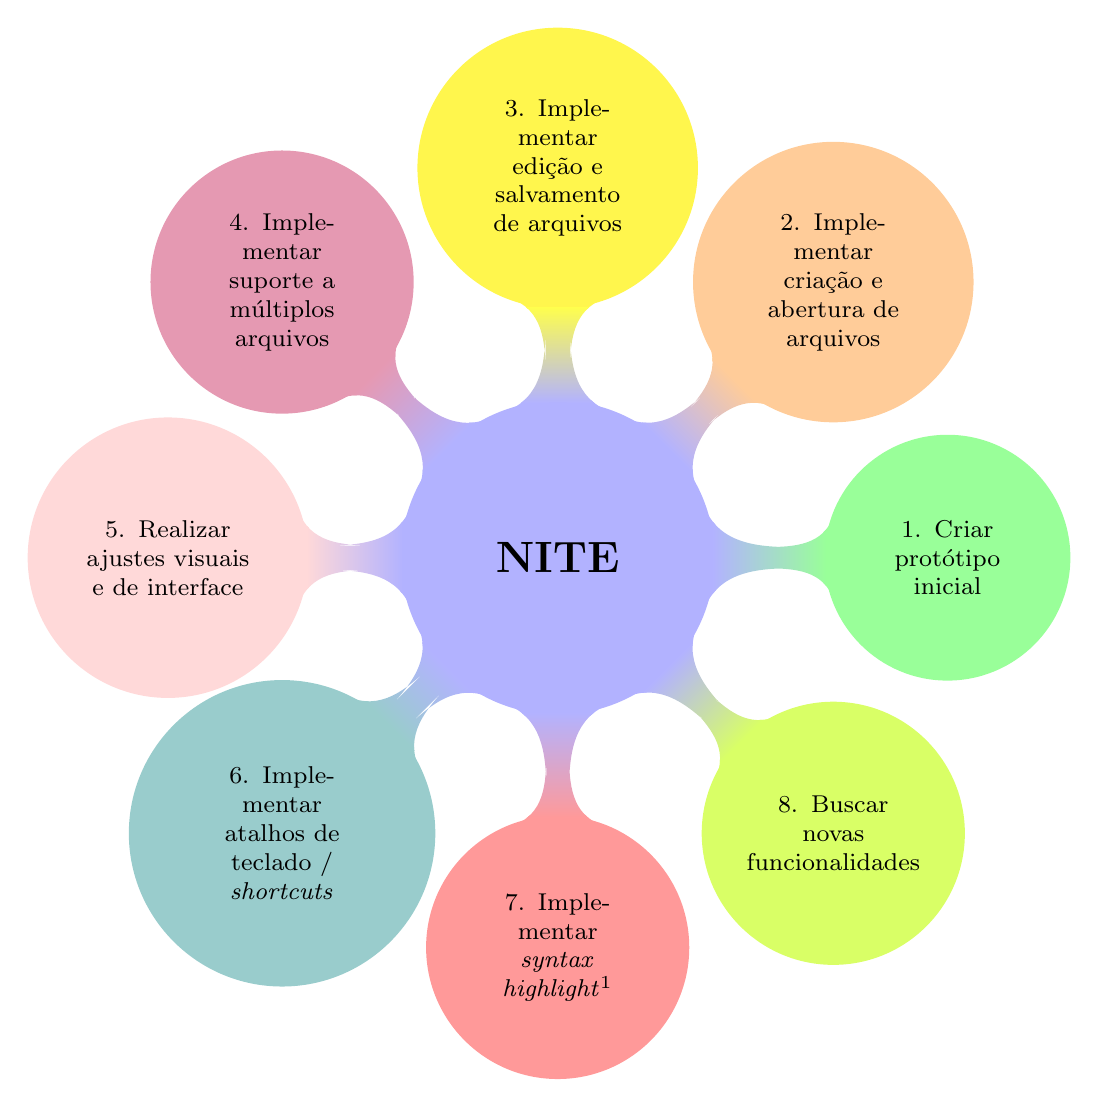
\begin{tikzpicture}[scale=1.1, transform shape]
        \path[
            mindmap,
            concept color=blue!30,
            text=black,
            level 1/.append style={sibling angle=45, level distance=4.5cm},
            every node/.style={align=center}
        ]
            node[concept, font=\Large\bfseries, minimum size=2.5cm] {NITE}
            [clockwise from=0]
            child[concept color=green!40, grow=0]
            { node[concept, font=\footnotesize, minimum size=2.8cm] {1. Criar\\protótipo\\inicial} }
            child[concept color=orange!40, grow=45]
            { node[concept, font=\footnotesize, minimum size=3.2cm] {2. Implementar\\criação e\\abertura de\\arquivos} }
            child[concept color=yellow!70, grow=90]
            { node[concept, font=\footnotesize, minimum size=3.2cm] {3. Implementar\\edição e\\salvamento\\de arquivos} }
            child[concept color=purple!40, grow=135]
            { node[concept, font=\footnotesize, minimum size=3cm] {4. Implementar\\suporte a\\múltiplos\\arquivos} }
            child[concept color=pink!60, grow=180]
            { node[concept, font=\footnotesize, minimum size=3.2cm] {5. Realizar\\ajustes visuais\\e de interface} }
            child[concept color=teal!40, grow=225]
            { node[concept, font=\footnotesize, minimum size=3.5cm] {6. Implementar\\atalhos de\\teclado /\\\textit{shortcuts}} }
            child[concept color=red!40, grow=270]
            { node[concept, font=\footnotesize, minimum size=3cm] {7. Implementar\\\textit{syntax}\\\textit{highlight}\footnotemark[1]} }
            child[concept color=lime!60, grow=315]
            { node[concept, font=\footnotesize, minimum size=3cm] {8. Buscar\\novas\\funcionalidades} };
    \end{tikzpicture}
    \footnotetext[1]{Destaque de sintaxe}
\end{center}

Consequentemente, isso permite testes cuidadosos das funcionalidades implementadas,
além de possibilitar ajustes sempre que necessário de forma ágil e controlada.

Descrito na sessão anterior, a linguagem de desenvolvimento que mais se adequa a
proposta do projeto foi a linguagem C, por sua confiabilidade e utilização
continua em projetos semelhantes. Nessa lógica a biblioteca utilizada para manipulação
de terminal foi a Ncurses, muito bem fundamentada e completa de funcionaidades
que serão aproveitadas ao máximo. Como ferramentas auxiliares, o uso do Git para
versionamento de arquivos, o editor Zed como IDE principal de desenvolvimento e o
ambiente Linux com o terminal BlackBox para testes. Vale ressaltar aqui o uso do
GCC\footnote{Coleção de compiladores do projeto GNU} como compilador.

Cada etapa do desenvolvimento é realizada em paralelo a análises e estudos do código-fonte
de outros editores, como o NeoVim, com ênfase no código do Nano, editor que
serviu de base para o NITE. Já na implementação de destaque de sintaxe, a
biblioteca Tree-Sitter será estudada e utilizada, gerando árvores de sintaxe abstratas
que ajudarão na implementação de destaque de sintaxe para o projeto \cite{tree-sitter}.               % FEITO	- REVISÃO: Ortográfica
    \chapter{Resultados Parciais}
\label{cap:04}

Baseado no cronograma proposto, esta sessão tem como objetivo discutir os resultados parciais de cada nó do diagrama anteriormente apresentado.

\section{Desenvolvimento}

Idealizando o projeto como um todo e utilizando a ferramenta Obsidian\footnote{Disponível em: https://obsidian.md/} como notas, foi possível
compreender melhor o projeto e planejar novas implementações no NITE. Com a ideia geral do editor finalizada, como deverá se comportar e a forma
como os comandos do editor irão funcionar (além de seus dois modos) entre outras funcionalidades descritas, a criação de protótipos se fez necessário
para a complementação do projeto final.

\subsection{Interface Inicial}

Diferente do editor NANO, que ao ser chamado sozinho\footnote{Quando nenhum arquivo é aberto ou criado ao ser chamado via terminal}
abre diretamente na tela de edição, com informações de versão no topo e comandos abaixo, foi idealizado criar uma ``tela inicial'' para o NITE,
como as vistas no Vim e seus derivados, a diferença é que os mesmos são altamente personalizáveis, funcionalidade que não será implementada.

\FloatBarrier
\begin{figure}[!htbp]
    \centering
    \caption{Tela inicial do NITE}
    \includegraphics[scale=0.3]{imagens/NITE.png}
    \\\textbf{Fonte: O autor} \label{fig:NITE}
\end{figure}
\FloatBarrier

Como mostra a Figura \ref{fig:NITE}, as ideias anteriormente descritas no Obsidian ganharam forma, obtendo inicialmente esta tela de apresentação,
onde o usuário tem acesso a comandos rápidos (e essenciais) para o funcionamento de qualquer editor: criar ou abrir arquivo.
Ainda, além do comando de saída do editor, o protótipo possui o comando de ajuda, que deverá abrir um guia de comandos que serão
implementados para navegação e funcionamento do NITE, além de explicar os modos leitura e edição.

\subsection{Criação e abertura de arquivo}

Passando para o proximo nó do diagrama e essencial para funcionamento de qualquer editor de texto, o próximo passo foi a implementação
de criação de arquivo. Com um ``\textit{extends}''\footnote{Extende outra funcionalidade}, a implementação dessa funcionalidade
também conta com a edição de arquivo.

Ao criar um arquivo no NITE, o mesmo pergunta o nome que o usuário pretende dar ao \textit{file}\footnote{Arquivo em inglês} (posteriormente poderá ser editado),
podendo ou não conter uma extensão válida. As extenções aceitas e não aceitas podem ser vistas na tabela abaixo:

\begin{table}[h]
    \centering
    \caption{Extensões de arquivos aceitos e bloqueados pelo editor NITE}
    \renewcommand{\arraystretch}{1.3}
    \setlength{\tabcolsep}{8pt}
    \begin{tabular}{@{}p{3.5cm}p{5.2cm}p{5.2cm}@{}}
        \toprule
        \textbf{Categoria} &
        \textbf{Extensões válidas} &
        \textbf{Extensões não válidas} \\
        \midrule
        \textbf{Texto plano} &
        .txt, .md, .csv, .log &
        – \\

        \textbf{Código-fonte} &
        Arquivos de texto contendo código de linguagens de programação
        (ex.: .c, .cpp, .java, .py, .js, .html, .css, .json, .xml, etc.) &
        – \\

        \textbf{Configurações} &
        .ini, .conf, .properties, .toml &
        – \\

        \textbf{Scripts executáveis} &
        .sh, .bat, .ps1, .cmd &
        – \\

        \textbf{Executáveis / Binários} &
        – &
        .exe, .dll, .so, .bin, .out, .app \\

        \textbf{Mídia (imagens / áudio / vídeo)} &
        – &
        .png, .jpg, .jpeg, .gif, .bmp, .mp3, .mp4, .wav \\

        \textbf{Compactados} &
        – &
        .zip, .rar, .tar, .gz, .7z \\

        \textbf{Documentos binários} &
        – &
        .doc, .docx, .pptx, .xlsx, .pdf \\

        \textbf{Imagens de disco} &
        – &
        .iso, .img \\
        \bottomrule
    \end{tabular}
\end{table}

Caso uma das extensão não aceitas seja chamada, o editor exibirá um erro e solicitará que o usuário crie um arquivo válido. Em caso do usuário
não fornecer uma extensão, o editor continuará o processo normalmente passando para a página de edição.

Inicialmente, o protótipo apresenta as seguintes informações no topo do arquivo: nome do arquivo sendo editado, F1 para salvar e F2 para sair
do editor. Ambas as funcionalidades abrirão uma nova janela que confirma a saída ou o salvamento do arquivo.

\FloatBarrier
\begin{figure}[!htbp]
    \centering
    \caption{NITE confirmando o salvamento de arquivo}
    \includegraphics[scale=0.3]{imagens/ConfirmSave.png}
    \\\textbf{Fonte: O autor} \label{fig:ConfirmSave}
\end{figure}
\FloatBarrier

Caso o usuário resolva sair do editor sem salvar o arquivo, uma mensagem é exibida no terminal após a saída. Caso o arquivo foi salvo, após a saída do editor, outra mensagem é exibida. Para essa funcionalidade, a biblioteca \textit{panel}\footnote{Faz parte do conjunto de bibliotecas \textit{ncurses}, usada para criar interfaces de texto como janelas, menus e painéis sobrepostos} foi utilizada.

\section{Repositório do Github}

O código base do editor e este documento se encontram disponíveis no link do Github: \url{https://github.com/Sunref/nite}

\section{Cronograma do Trabalho}

Segue abaixo o cronograma de trabalho das atividades realizadas.

\FloatBarrier
\begin{figure*}[!htbp]
	\centering
	\includegraphics[scale=0.4]{imagens/cronograma.png}
\end{figure*}
\FloatBarrier

\begin{enumerate}
	\item Atividade 01: Implementação do protótipo inicial;
	\item Atividade 02: Criação e abertura de arquivos;
	\item Atividade 03: Edição e Salvamento de arquivo;
	\item Atividade 04: Suporte a múltiplos arquivos;
	\item Atividade 05: Atalhos de teclado;
	\item Atividade 06: Ajustes visuais e de interface;
	\item Atividade 07: Destaque de sintaxe;
	\item Atividade 08: Buscar outras funcionalidades para implementação.
\end{enumerate}		% FEITO	- REVISÃO: Ortográfica
    \chapter{Conclusões e Recomendações}
\label{cap:05}

O NITE se encontra em fase de desenvolvimento, com avanços significativos de suas principais funcionalidades.
Apesar do progresso, ainda se faz necessário dar continuidade ao projeto, reservando espaço para futuras
implementações que irão contribuir para o funcionamento total do editor CLI. Ajustes referentes a interface e
usabilidade devem seguir em todos os passos (incluindo os de estágio avançado), seguindo de levantamentos e
apresentação de resultados, visando usabilidade. No decorrer dos proximos meses, pretende-se concluir sua fase de
testes e desenvolvimento, possibilitando a apresentação dos resultados finais, impactos e propostas de soluções.	% FEITO	- REVISÃO: Ortográfica

    % ----------------------------------------------------------
    % Referências bibliográficas
    % ----------------------------------------------------------
    \postextual
    \bibliography{referencias}
\end{document}